\def\nr{9. Aufgabenblatt}
\def\kopf{\\\hfill\normalsize\mdseries}
\documentclass[11pt,a4paper,fleqn]{scrartcl}
\usepackage{eurosym}
\usepackage{adjustbox}
%\usepackage{a4kopka}
\usepackage{amsmath,amssymb,amsthm,amsfonts}
\usepackage[utf8]{inputenc}
\usepackage{algorithmic,algorithm}
\usepackage{graphics,graphicx}
\usepackage{pgfplots,tikz}
\usepackage{enumerate}
\usepackage[ngerman]{babel}
% \usepackage[software]{mymacros}
%\usepackage{matrix}
\usepackage{hyperref}
% \usepackage{caption}
\usepackage{caption, subcaption}

\floatname{algorithm}{Algorithmus}
\renewcommand{\algorithmicrequire}{\textbf{Input:}}
\renewcommand{\algorithmicensure}{\textbf{Output:}}

%\usepackage{enumitem} 
%\textheight25cm
\textheight23cm
\topmargin-15mm
\oddsidemargin-5mm    %  -10mm
\textwidth17cm    %   18.8cm
\footskip0pt
\thispagestyle{empty}
\parindent0mm
\parskip0ex
\parskip0ex

\makeatletter
\DeclareOldFontCommand{\rm}{\normalfont\rmfamily}{\mathrm}
\DeclareOldFontCommand{\sf}{\normalfont\sffamily}{\mathsf}
\DeclareOldFontCommand{\tt}{\normalfont\ttfamily}{\mathtt}
\DeclareOldFontCommand{\bf}{\normalfont\bfseries}{\mathbf}
\DeclareOldFontCommand{\it}{\normalfont\itshape}{\mathit}
\DeclareOldFontCommand{\sl}{\normalfont\slshape}{\@nomath\sl}
\DeclareOldFontCommand{\sc}{\normalfont\scshape}{\@nomath\sc}
\makeatother

% \newcommand{\cg}[1]{{\color{blue} #1}}
% \newcommand{\cb}[1]{{\color{green} #1}}
% \newcommand{\cred}[1]{{\color{red} #1}}
% \newcommand{\cc}[1]{{\color{cyan} #1}}
% \newcommand{\cm}[1]{{\color{magenta} #1}}

\newcommand{\Aufgabe}[2][]{\par\bigskip{\sf\bfseries Aufgabe #2#1:}}
%\hspace{3em}{\small(#2 point\ifthenelse{#2>1}{s}{})}}\par\smallskip}
%\newcommand\aufgabe[2][~]{\par\bigskip{\sf\bfseries Aufgabe #1
%    \hspace{3em} \ifthenelse{\equal{#2}{~}}{}{(#2)}}\par\smallskip}
\usepackage{mymacros}

\begin{document}
{\sf Universit\"at Hamburg \hfill Wintersemester 2020/21 \\ Fachbereich Mathematik \\ Dr. Matthias Voigt}
\begin{center}
\ifthenelse{\equal{\nr}{no}}{\Large\sf\bfseries \kopf}{\Large\sf\bfseries Optimierung f\"ur Studierende der Informatik -- \nr.~\kopf}
\end{center}

\renewcommand{\tilde}{\widetilde}
\renewcommand{\hat}{\widehat}
\newcommand{\ri}{\mathrm{i}}
\renewcommand{\H}{\mathsf{H}}
\newcommand{\T}{\mathsf{T}}


\subsection*{Präsenzaufgaben am 18./19.01.2021}

\Aufgabe[ (Matchingzahl)]{P1}
% Aufgabe P-1
Geben Sie einen zusammenhängenden Graphen $G$ mit 10 Kanten an, für den $m(G) = 3$ gilt.

\Aufgabe[ (perfekte Matchings)]{P2}
% Aufgabe P-2
Betrachten Sie den folgenden Graphen:
\begin{center}
 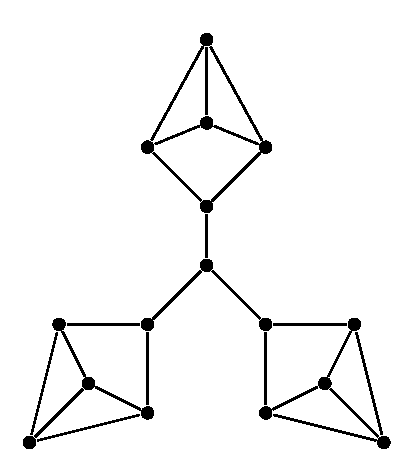
\includegraphics{fig9_1.pdf}
\end{center}
Besitzt dieser Graph ein perfektes Matching? Falls ja, so gebe man ein solches an; falls nein, so begründe man, wieso kein perfektes Matching existiert.

\Aufgabe[ (Matchingzahl und Knotenüberdeckungszahl)]{P3}
% Aufgabe P-3
\begin{enumerate}[a)]
% Aufgabe P-3a
\item Wie ist die Knotenüberdeckungszahl $c(G)$ eines Graphen $G$ definiert?
% Aufgabe P-3b
\item Begründen Sie (kurz), weshalb $m(G) \leq c(G)$ für jeden Graphen $G$ gilt.
% Aufgabe P-3c
\item Geben Sie einen Graphen $G$ an, für den $m(G) < c(G)$ gilt.
% Aufgabe P-3d
\item Kann die Differenz $c(G) - m(G)$ beliebig groß werden?
\end{enumerate}


\subsection*{Hausaufgaben bis zum 27.01.2021 (12:00 Uhr)}
\emph{Bitte reichen Sie Ihre Hausaufgaben in festen Zweier- oder Dreiergruppen bei Moodle ein. Bitte laden Sie ausschließlich \textbf{PDF-Dokumente} hoch, andernfalls können Ihre Hausaufgaben nicht korrigiert werden.}

\Aufgabe[ (maximale Matchings und minimale Knotenüberdeckungen, 10 Punkte)]{H1}
Bestimmen Sie für die beiden unten angegebenen Graphen jeweils ein Matching mit maximaler Kantenzahl sowie eine minimale Knotenüberdeckung. Verwenden Sie hierzu den Algorithmus von Edmonds und Karp, wobei die folgende Regel zu beachten ist: Gibt es mehrere Kandidaten für den nächsten zu markierenden Knoten, so sind Knoten mit kleinerem Index vorzuziehen.

\textbf{Hinweis}: Sie müssen nicht mehr das Flussnetzwerk explizit formulieren. Zudem können Sie mehrere Iterationen in einer Zeichnung zusammenfassen, falls sich dies anbietet (ähnlich wie in Beispiel 2 aus Vorlesung 9).

\begin{enumerate}[a)]
 \item\begin{minipage}[t]{\linewidth}
          \raggedright
          \adjustbox{valign=t}{%
%\begin{center}
 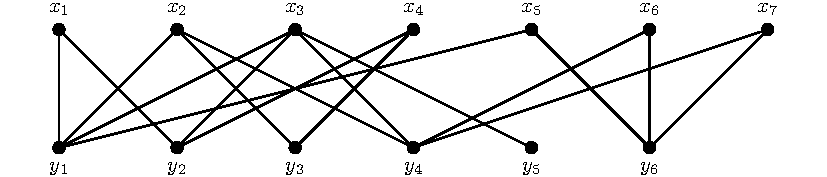
\includegraphics{fig9_2.pdf}
 }
 \end{minipage}
 \medskip
\item\begin{minipage}[t]{\linewidth}
          \raggedright
          \adjustbox{valign=t}{%
%\begin{center}
 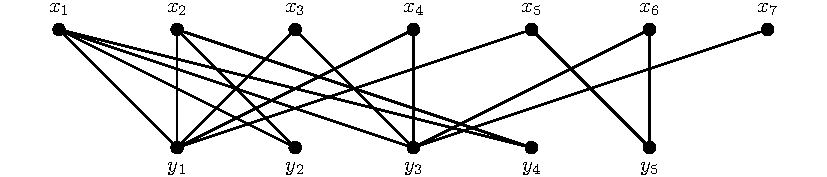
\includegraphics{fig9_3.pdf}
 }
 \end{minipage}
\end{enumerate}
\end{document}
